\chapter{Teorias da velocidade de reação}\label{ch:b3:rate-theories}

Em 2017 foi aprovado um medicamento cuja única diferença em relação a um mais
antigo é que os seis átomos de hidrogênio de seus dois grupos metoxila são
átomos de deutério. O fígado degrada o fármaco cortando exatamente essas
ligações C--H, e uma ligação C--D é cortada várias vezes mais devagar: a
molécula pesada permanece mais tempo no sangue e é tomada em doses menores e
menos frequentes. Nada na lei de Arrhenius explica por que um nêutron em um
núcleo deveria desacelerar uma reação. Este capítulo deduz as constantes de
velocidade a partir de propriedades moleculares: primeiro a partir das
colisões, depois a partir da forma da \omterm{def:b3:computational-chemistry:pes}{superfície de energia potencial} e das
funções de partição da \omterm{def:b3:rate-theories:tst}{teoria do estado de transição}, que prevê o tamanho
desses efeitos isotópicos; termina com as reações em solução, onde o solvente
impõe um limite de velocidade.

\begin{recall}
O volume do 1.º ano definiu a constante de velocidade, a lei de Arrhenius $k =
A\eu^{-E_a/RT}$ com sua energia de ativação e seu fator pré-exponencial, as
etapas elementares, o estado de transição, o perfil de energia ao longo da
coordenada de reação e o postulado de Hammond. O volume do 2.º ano definiu a
força iônica e os coeficientes de atividade, com a lei limite de Debye--Hückel
$\log\gamma_i = -Az_i^2\sqrt I$ ($A \approx
0.51$ em água a \qty{25}{\celsius}), e ajustou retas por mínimos quadrados. O
\cref{ch:b3:computational-chemistry} introduziu as \omterm{def:b3:computational-chemistry:pes}{superfícies de energia
potencial}; os \cref{ch:b3:partition-functions,ch:b3:statistical-thermo-applied}
calcularam constantes de equilíbrio a partir das funções de partição e das
\omterm{def:b3:quantum-model-systems:oscillator}{energias do ponto zero}. Da física: a distribuição de Maxwell--Boltzmann das
velocidades moleculares e a lei de Fick da difusão.
\end{recall}

\begin{omfigure}
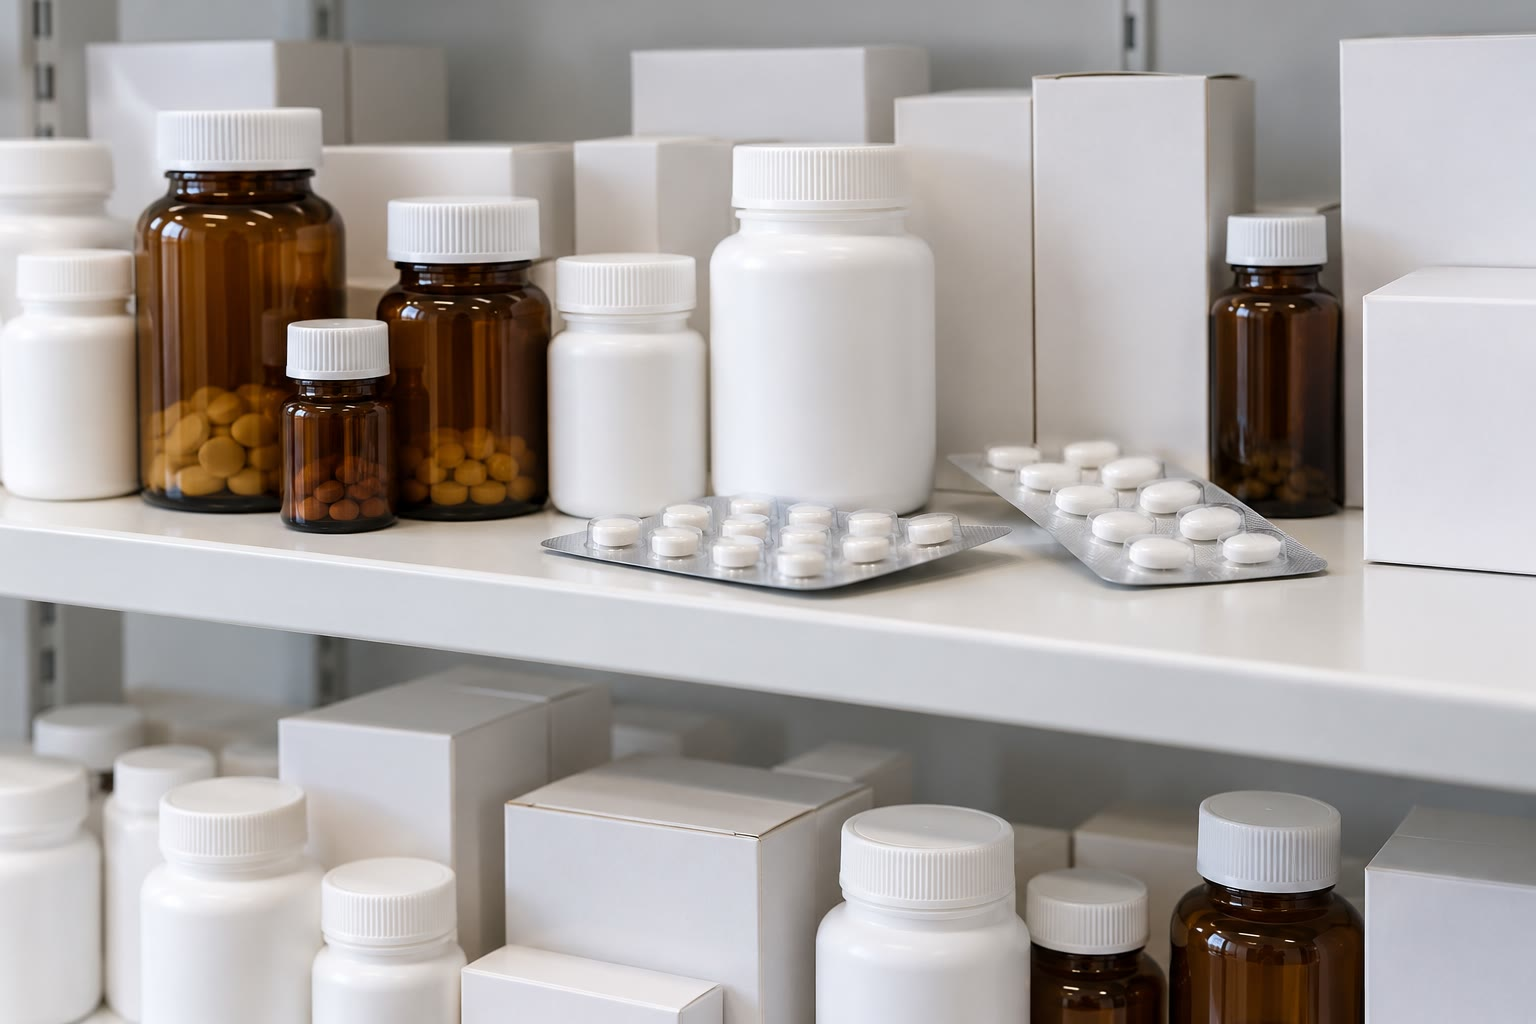
\includegraphics[width=0.6\linewidth]{images/book4/ai/b3-12-pharmacy.jpg}

{\small Medicamentos na prateleira de uma farmácia. Substituir o hidrogênio por
deutério nas ligações que o fígado ataca primeiro pode prolongar o tempo que um
fármaco permanece no organismo.}
\end{omfigure}

\section{A teoria das colisões}

Duas moléculas em um gás só podem reagir se se encontrarem. Modele-as como esferas
rígidas de diâmetros $d_{\mathrm A}$ e $d_{\mathrm B}$: elas colidem quando seus centros passam a menos de $d =
\frac12(d_{\mathrm A} + d_{\mathrm B})$ um do outro.

\begin{definition}[Seção eficaz de colisão, fator estérico]\label{def:b3:rate-theories:collision}
A \emph{seção eficaz de colisão}\index{secao eficaz de colisao@seção eficaz de colisão} de duas moléculas
é a área $\sigma = \pi d^2$ do disco, perpendicular à sua velocidade relativa,
dentro do qual o centro de uma deve passar para atingir a outra. O
\emph{fator estérico}\index{fator esterico@fator estérico} $P$ é a razão entre o fator
pré-exponencial medido de uma reação e o previsto pela teoria das colisões.
\end{definition}

\begin{omfigure}
\begin{tikzpicture}[font=\small, >=Stealth]
  \shade[ball color=omDef!40] (0,0) circle (0.45);
  \node at (0,0) {A};
  \draw[black!50, dashed] (-0.0,0.85) -- (5.2,0.85) (-0.0,-0.85) -- (5.2,-0.85);
  \draw[black!60] (0,0) ellipse (0.25 and 0.85);
  \draw[<->] (-0.45,0) -- (-0.45,0.85) node[midway, left] {$d$};
  \shade[ball color=omThm!40] (3.3,0.55) circle (0.4);
  \node at (3.3,0.55) {B};
  \shade[ball color=omThm!20] (4.6,1.45) circle (0.4);
  \node at (4.6,1.45) {B};
  \draw[->, thick] (0.6,0) -- (2.2,0) node[midway, below] {$v_{\mathrm{rel}}\,\Delta t$};
  \node[anchor=west, align=left, font=\scriptsize] at (5.3,0) {cilindro de\\ seção\\ $\sigma = \pi d^2$};
  \node[font=\scriptsize, anchor=south] at (3.3,1.0) {atingida};
  \node[font=\scriptsize, anchor=south] at (4.6,1.9) {errada};
\end{tikzpicture}

{\small O cilindro de colisão. Movendo-se com a velocidade relativa $v_{\mathrm{rel}}$, a molécula A
varre, em um tempo $\Delta t$, um cilindro de seção $\sigma = \pi d^2$, com $d$ a soma dos dois
raios; toda B cujo centro esteja dentro dele é atingida.}
\end{omfigure}

\begin{theorem}[Constante de velocidade da teoria das colisões]\label{thm:b3:rate-theories:collision}
Se toda colisão cuja energia cinética ao longo da linha dos centros excede um
limiar $E_0$ (por mol) leva à reação, a constante de velocidade de $\mathrm{A + B} \to$
produtos é
\[
  k = \sigma\bar v_{\mathrm{rel}}N_A\,\eu^{-E_0/RT}, \qquad \bar v_{\mathrm{rel}} = \sqrt{\frac{8kT}{\pi\mu}},\
  \mu = \frac{m_{\mathrm A}m_{\mathrm B}}{m_{\mathrm A} + m_{\mathrm B}} .
\]
\end{theorem}

\begin{proof}[Demonstração parcial]
Em um tempo $\Delta t$, uma molécula A varre um volume $\sigma v_{\mathrm{rel}}\Delta t$ e atinge as
$n_{\mathrm B}\sigma v_{\mathrm{rel}}\Delta t$ moléculas B que ele contém: a frequência de colisões por unidade de volume
é $\sigma\bar v_{\mathrm{rel}}n_{\mathrm A}n_{\mathrm B}$, com $\bar v_{\mathrm{rel}}$ a velocidade relativa média dada pela
distribuição de Maxwell--Boltzmann (admitida da física, com a \omterm{def:b3:quantum-model-systems:oscillator}{massa
reduzida}). Ponderar cada colisão por sua velocidade e conservar aquelas cuja
energia ao longo da linha dos centros excede o limiar deixa a fração
$\eu^{-E_0/RT}$ da frequência de colisões (a integração sobre o parâmetro de impacto é
admitida). Converter densidades numéricas em concentrações molares multiplica por
$N_A$.
\end{proof}

Como $\bar v_{\mathrm{rel}} \propto \sqrt T$, a energia de ativação $E_a = RT^2\,\dd\ln k/\dd T$ vale $E_0 + \frac12RT$,
próxima do limiar. O fator pré-exponencial é da ordem de
$10^{11}$~\unit{L.mol^{-1}.s^{-1}} para moléculas pequenas. Os fatores medidos são
muitas vezes bem menores: $P \ll 1$ para moléculas que precisam se encontrar em
uma orientação particular, e a seção eficaz não tem valor único para moléculas
reais, que não são esferas rígidas. A teoria das colisões dá a ordem de grandeza
e a dependência com a temperatura; ela não pode dar $E_0$, que exige a \omterm{def:b3:computational-chemistry:pes}{superfície
de energia potencial}.

\section{Superfícies de energia potencial}

A reação $\mathrm{H_A + H_BH_C \to H_AH_B + H_C}$ é a mais simples que existe. Para uma
aproximação colinear, a energia depende de duas distâncias, $r_{\mathrm{AB}}$ e $r_{\mathrm{BC}}$, e pode ser
desenhada como um mapa.

\begin{definition}[Ponto de sela, caminho de energia mínima]\label{def:b3:rate-theories:saddle}
Um \emph{ponto de sela}\index{ponto de sela} de uma \omterm{def:b3:computational-chemistry:pes}{superfície de energia potencial} é um
ponto onde o gradiente se anula e a energia é máxima ao longo de uma direção e
mínima ao longo de todas as outras. O \emph{caminho de energia mínima}\index{caminho de energia minima@caminho de energia mínima}
é o caminho de máxima descida do ponto de sela até os vales dos reagentes e
dos produtos; seu comprimento medido ao longo dele é a coordenada de reação, e
o ponto de sela é o estado de transição.
\end{definition}

\begin{omfigure}
\begin{tikzpicture}
\begin{axis}[ompes, width=0.62\linewidth, xmin=0.4, xmax=3.0, ymin=0.4, ymax=3.0,
  xlabel={$r_{\mathrm{AB}}$ / \AA}, ylabel={$r_{\mathrm{BC}}$ / \AA},
  colorbar, colorbar style={ylabel={$E$ / eV}, ylabel style={font=\small},
  yticklabel style={font=\small}}, point meta min=-4.7, point meta max=-0.8]
\addplot3[contour prepared={labels=false}, thick] table {figdata/out/bachelor-3-pes-collinear-contours.dat};
\addplot3[ompath] table[x=x, y=y, z expr=0] {figdata/out/bachelor-3-pes-collinear-mep.dat};
\node[omsaddle] at (axis cs:0.918,0.918,0) {};
\node[font=\small, anchor=south west] at (axis cs:0.95,0.95,0) {sela};
\node[font=\small, anchor=west, fill=white, fill opacity=0.85, text opacity=1, inner sep=1.5pt] at (axis cs:2.05,1.0,0) {$\mathrm{H_A + H_BH_C}$};
\node[font=\small, anchor=west, fill=white, fill opacity=0.85, text opacity=1, inner sep=1.5pt] at (axis cs:0.95,2.55,0) {$\mathrm{H_AH_B + H_C}$};
\node[font=\small, anchor=north east] at (axis cs:2.95,2.95,0) {$\ce{H + H + H}$};
\end{axis}
\end{tikzpicture}

{\small Uma superfície de energia potencial-modelo para $\ce{H + H2}$ colinear (forma LEPS
construída a partir da curva de Morse de \ce{H2}, com um parâmetro de Sato de 0.17
escolhido como constante do modelo). Curvas de nível de \qty{-4.65}{eV} a \qty{-0.8}{eV},
com o zero de energia para três átomos separados; os vales ficam a \qty{-4.75}{eV}, a
profundidade do poço de \ce{H2}. Tracejado: o \omterm{def:b3:rate-theories:saddle}{caminho de energia mínima}, que atravessa
a sela simétrica em $r_{\mathrm{AB}} = r_{\mathrm{BC}} = \qty{0.92}{\angstrom}$,
\qty{0.27}{eV} acima dos vales nesse modelo.}
\end{omfigure}

O caminho sobe do vale dos reagentes, onde $r_{\mathrm{BC}}$ permanece perto do comprimento
de ligação de \ce{H2} enquanto A se aproxima, atravessa a sela e desce ao vale dos
produtos. Na sela, as duas ligações estão esticadas a \qty{0.92}{\angstrom}: a antiga
ligação está meio rompida e a nova meio formada, e o custo energético desse
compromisso é a barreira. Para a reação simétrica, a sela fica na diagonal; para
uma reação exotérmica, ela se desloca para o vale dos reagentes (uma barreira
precoce, um estado de transição semelhante aos reagentes, como diz o postulado de
Hammond), e para uma endotérmica, para o vale dos produtos (uma barreira tardia).
A posição decide que energia ajuda: a energia de translação, dirigida ao longo do
vale de entrada, leva as moléculas por cima de uma barreira precoce; uma barreira
tardia, depois de uma curva, é transposta mais facilmente com energia vibracional
na ligação que se rompe. Essas são as regras de Polanyi, confirmadas por
experimentos com feixes moleculares.

\section{A teoria do estado de transição}

\begin{definition}[Complexo ativado]\label{def:b3:rate-theories:activated-complex}
O \emph{complexo ativado}\index{complexo ativado} de uma etapa elementar é o
conjunto das configurações do sistema reagente em uma fatia fina em torno do
\omterm{def:b3:rate-theories:saddle}{ponto de sela}, perpendicular ao \omterm{def:b3:rate-theories:saddle}{caminho de energia mínima}; ele é tratado como
uma espécie $\ce{AB^{\ddagger}}$, com sua própria função de partição.
\end{definition}

\begin{definition}[Teoria do estado de transição, coeficiente de transmissão]\label{def:b3:rate-theories:tst}
A \emph{teoria do estado de transição}\index{teoria do estado de transicao@teoria do estado de transição} supõe que
os \omterm{def:b3:rate-theories:activated-complex}{complexos ativados} estão em equilíbrio com os reagentes, que todo complexo que
atravessa a região da sela em direção aos produtos chega a formá-los, e que o
movimento ao longo da coordenada de reação é uma translação livre. O
\emph{coeficiente de transmissão}\index{coeficiente de transmissao@coeficiente de transmissão} $\kappa \le 1$ corrige
os complexos que recruzam de volta para os reagentes.
\end{definition}

\begin{theorem}[Equação de Eyring]\label{thm:b3:rate-theories:eyring}
Para uma etapa elementar $\mathrm{A + B} \to \mathrm{AB}^{\ddagger} \to$ produtos,
\[
  k = \kappa\frac{k_BT}{h}\overline{K}{}^{\ddagger}, \qquad
  \overline{K}{}^{\ddagger} = \frac{\bar q^{\ddagger}/N_A}{(q_{\mathrm A}/N_A)(q_{\mathrm B}/N_A)}\,\eu^{-\Delta E_0^{\ddagger}/RT},
\]
onde $\bar q^{\ddagger}$ é a função de partição do \omterm{def:b3:rate-theories:activated-complex}{complexo ativado} sem o movimento ao
longo da coordenada de reação, os $q$ são funções de partição molares por unidade
de volume, e $\Delta E_0^{\ddagger}$ é a altura do nível do ponto zero do complexo acima
do dos reagentes. Na forma termodinâmica, com $c^\circ = \qty{1}{mol/L}$ e a
molecularidade $m$,
\[
  k = \kappa\frac{k_BT}{h}(c^\circ)^{1-m}\,\eu^{\Delta^{\ddagger}S^\circ/R}\,\eu^{-\Delta^{\ddagger}H^\circ/RT}.
\]
Esse enunciado é a \emph{equação de Eyring}\index{equacao de Eyring@equação de Eyring}; $k_B$ é a
constante de Boltzmann, escrita assim para evitar confusão com $k$.
\end{theorem}

\begin{proof}
Quase equilíbrio: $[\ce{AB^{\ddagger}}] = K^{\ddagger}[\mathrm A][\mathrm B]$, com $K^{\ddagger}$ obtido das funções de partição
(\cref{thm:b3:statistical-thermo-applied:k-from-q}, escrito com concentrações).
Das vibrações do complexo, uma é o movimento ao longo da coordenada de reação:
uma vibração muito frouxa de frequência $\nu \ll k_BT/h$, cuja função de partição
é $k_BT/h\nu$ (o limite de alta temperatura da
\cref{prop:b3:partition-functions:q-vib}); logo $q^{\ddagger} = \bar q^{\ddagger}k_BT/h\nu$. Os
complexos atravessam em direção aos produtos com a frequência $\nu$ desse movimento,
logo a velocidade é $\nu[\ce{AB^{\ddagger}}] = \nu\frac{k_BT}{h\nu}\overline{K}{}^{\ddagger}[\mathrm A][\mathrm B]$: a frequência desconhecida $\nu$ se cancela. Escrever
$\overline{K}{}^{\ddagger} = (c^\circ)^{1-m}\eu^{-\Delta^{\ddagger}G^\circ/RT}$ e $\Delta^{\ddagger}G^\circ = \Delta^{\ddagger}H^\circ - T\Delta^{\ddagger}S^\circ$ dá a
segunda forma, com $\kappa$ inserido para levar em conta o recruzamento.
\end{proof}

O fator $k_BT/h$ vale \qty{6.2e12}{s^{-1}} a \qty{298}{K}: a velocidade de uma etapa
unimolecular sem barreira e sem perda de entropia. Tudo o que é específico da
reação está nas grandezas de ativação.

\begin{definition}[Energia de Gibbs, entalpia e entropia de ativação]\label{def:b3:rate-theories:activation}
A \emph{energia de Gibbs de ativação}\index{energia de Gibbs de ativacao@energia de Gibbs de ativação}
$\Delta^{\ddagger}G^\circ$, a \emph{entalpia de ativação}\index{entalpia de ativacao@entalpia de ativação} $\Delta^{\ddagger}H^\circ$ e a
\emph{entropia de ativação}\index{entropia de ativacao@entropia de ativação} $\Delta^{\ddagger}S^\circ$ de uma etapa
elementar são a energia de Gibbs, a entalpia e a entropia padrão de formação do
\omterm{def:b3:rate-theories:activated-complex}{complexo ativado} (sem seu movimento ao longo da coordenada de reação) a partir dos
reagentes, definidas pela \omterm{thm:b3:rate-theories:eyring}{equação de Eyring}.
\end{definition}

\begin{proposition}[Energia de ativação e entalpia de ativação]\label{prop:b3:rate-theories:ea-dh}
Para uma reação em solução, $E_a = \Delta^{\ddagger}H^\circ + RT$; para uma reação bimolecular em fase gasosa,
$E_a = \Delta^{\ddagger}H^\circ + 2RT$.
\end{proposition}

\begin{proof}
$E_a = RT^2\,\dd\ln k/\dd T$, e $\ln k = \ln T + \Delta^{\ddagger}S^\circ/R - \Delta^{\ddagger}H^\circ/RT + $ const: $E_a =
RT + \Delta^{\ddagger}H^\circ$ quando os parâmetros de ativação não variam com $T$. Em solução,
é o resultado. Em fase gasosa, a relação de van 't Hoff para $K^{\ddagger}$ escrita
em concentrações envolve a energia interna, $\Delta^{\ddagger}U^\circ = \Delta^{\ddagger}H^\circ - \Delta n^{\ddagger}RT$
com $\Delta n^{\ddagger} = 1 - m$: para $m = 2$, $E_a = \Delta^{\ddagger}H^\circ + 2RT$.
\end{proof}

A \omterm{def:b3:rate-theories:activation}{entropia de ativação} lê a estrutura do estado de transição. Duas moléculas
que se combinam em um único complexo perdem liberdade de translação e de
rotação: $\Delta^{\ddagger}S^\circ$ é fortemente negativa, de $-50$ a $-150$ \unit{J.K^{-1}.mol^{-1}}, para
as etapas associativas e os estados de transição cíclicos. Uma molécula que
afrouxa uma ligação a caminho da dissociação ganha liberdade: $\Delta^{\ddagger}S^\circ > 0$.

\begin{proposition}[Incertezas-padrão de uma reta ajustada]\label{prop:b3:rate-theories:slope-uncertainty}
Para uma reta de mínimos quadrados $y = a + bx$ através de $n$ pontos cujos $y$ têm
erros independentes de mesma variância, estimada por $s^2 = \sum_i(y_i - a - bx_i)^2/(n - 2)$,
a inclinação e o intercepto têm as incertezas-padrão
\[
  s_b = \frac{s}{\sqrt{\sum_i(x_i - \bar x)^2}}, \qquad
  s_a = s\sqrt{\frac1n + \frac{\bar x^2}{\sum_i(x_i - \bar x)^2}} .
\]
\end{proposition}

\begin{proof}
$b = \sum_i(x_i - \bar x)y_i/S_{xx}$, com $S_{xx} = \sum_i(x_i - \bar x)^2$, é uma combinação linear de
$y_i$ independentes de variância $\sigma^2$: sua variância é $\sigma^2\sum_i(x_i - \bar x)^2/S_{xx}^2 = \sigma^2/S_{xx}$.
Do mesmo modo, $a = \bar y - b\bar x$, e $\bar y$ e $b$ não são correlacionados (sua covariância é
$\sigma^2\sum_i(x_i - \bar x)/(nS_{xx}) = 0$), logo $\operatorname{var}a = \sigma^2/n + \bar x^2\sigma^2/S_{xx}$. Substituir $\sigma^2$
por sua estimativa $s^2$ (o divisor $n - 2$ leva em conta os dois parâmetros
ajustados, admitido) dá o resultado.
\end{proof}

\begin{method}[Um gráfico de Eyring com incertezas]\label{met:b3:rate-theories:eyring-plot}
\begin{enumerate}
  \item Meça $k$ em cinco temperaturas ou mais, distribuídas sobre 30 a \qty{40}{K}.
  \item Trace $y = \ln(k/T)$ em função de $x = 1/T$ e ajuste a reta de mínimos quadrados $y = a + bx$.
  \item $\Delta^{\ddagger}H^\circ = -Rb$ e $\Delta^{\ddagger}S^\circ = R[a - \ln(k_B/h)]$ ($\ln(k_B/h) = 23.760$ com $k$ em
        \unit{s^{-1}}).
  \item Suas incertezas-padrão são $Rs_b$ e $Rs_a$; um intervalo de confiança de 95\,\%
        as multiplica pelo $t$ de Student para $n - 2$ graus de liberdade (3.18 para
        cinco pontos).
  \item O intercepto fica muito fora do intervalo medido, em $1/T = 0$: $\Delta^{\ddagger}S^\circ$
        é sempre muito menos precisa que $\Delta^{\ddagger}H^\circ$, e os dois erros são
        correlacionados.
\end{enumerate}
\end{method}

\begin{omfigure}
\begin{tikzpicture}
\begin{axis}[width=0.74\linewidth, height=6.2cm, xmin=3.12, xmax=3.62, ymin=-12.8, ymax=-6.4,
  axis lines=left, xlabel={$1000\,\mathrm K/T$}, ylabel={$\ln\bigl(k/(\mathrm s^{-1}\,\mathrm K^{-1})\bigr)$},
  tick label style={font=\small}, label style={font=\small},
  legend style={font=\scriptsize, draw=none, fill=white, fill opacity=0.85, text opacity=1,
  at={(0.98,0.98)}, anchor=north east}, legend cell align=left]
\addplot[omDef, thick] table[x=invT, y=fit] {figdata/out/bachelor-3-eyring-band-H.dat};
\addplot[omThm, thick] table[x=invT, y=fit] {figdata/out/bachelor-3-eyring-band-D.dat};
\addplot[omDef, thin, dashed, forget plot] table[x=invT, y=lo] {figdata/out/bachelor-3-eyring-band-H.dat};
\addplot[omDef, thin, dashed, forget plot] table[x=invT, y=hi] {figdata/out/bachelor-3-eyring-band-H.dat};
\addplot[omThm, thin, dashed, forget plot] table[x=invT, y=lo] {figdata/out/bachelor-3-eyring-band-D.dat};
\addplot[omThm, thin, dashed, forget plot] table[x=invT, y=hi] {figdata/out/bachelor-3-eyring-band-D.dat};
\addplot[only marks, mark=*, mark size=1.8pt, omDef, forget plot] table[x=invT, y=lnkT_H] {figdata/out/bachelor-3-eyring-points.dat};
\addplot[only marks, mark=square*, mark size=1.7pt, omThm, forget plot] table[x=invT, y=lnkT_D] {figdata/out/bachelor-3-eyring-points.dat};
\legend{fármaco \ce{OCH3}, fármaco \ce{OCD3}}
\end{axis}
\end{tikzpicture}

{\small Gráficos de Eyring das constantes de velocidade do problema de fim de semana
(dados do problema) para o fármaco e seu análogo deuterado, com as retas de
mínimos quadrados e suas faixas de confiança de 95\,\% (tracejadas, pouco mais
largas que as retas: os pontos se dispersam cerca de 1\,\%). As retas são
paralelas dentro de sua incerteza: a mesma \omterm{def:b3:rate-theories:activation}{entropia de ativação}, \omterm{def:b3:rate-theories:activation}{entalpias de
ativação} que diferem de cerca de \qty{5}{kJ/mol}.}
\end{omfigure}

\section{Efeitos isotópicos cinéticos}

\begin{definition}[Efeitos isotópicos cinéticos]\label{def:b3:rate-theories:kie}
O \emph{efeito isotópico cinético}\index{efeito isotopico cinetico@efeito isotópico cinético} de uma etapa é a
razão $k_{\mathrm{light}}/k_{\mathrm{heavy}}$ de suas constantes de velocidade para dois \omterm{def:b3:rovibrational-spectroscopy:rotational-constant}{isotopólogos}, na maioria
das vezes $k_{\mathrm H}/k_{\mathrm D}$. É um \emph{efeito isotópico cinético primário}\index{efeito isotopico cinetico primario@efeito isotópico cinético primário}
quando a ligação ao átomo substituído é formada ou rompida na etapa, e um
\emph{efeito isotópico cinético secundário}\index{efeito isotopico cinetico secundario@efeito isotópico cinético secundário}
quando não é.
\end{definition}

\begin{proposition}[Efeito isotópico cinético primário máximo]\label{prop:b3:rate-theories:primary-kie}
Se a vibração de estiramento de uma ligação X--H se torna a coordenada de reação,
de modo que sua \omterm{def:b3:quantum-model-systems:oscillator}{energia do ponto zero} se perde no estado de transição enquanto
todas as outras contribuições são as mesmas para H e D,
\[
  \frac{k_{\mathrm H}}{k_{\mathrm D}} = \exp\Bigl[\frac{hc(\tilde\nu_{\mathrm{XH}} - \tilde\nu_{\mathrm{XD}})}{2k_BT}\Bigr],
  \qquad \frac{\tilde\nu_{\mathrm{XH}}}{\tilde\nu_{\mathrm{XD}}} = \sqrt{\frac{\mu_{\mathrm{XD}}}{\mu_{\mathrm{XH}}}} .
\]
\end{proposition}

\begin{proof}
A \omterm{def:b3:computational-chemistry:pes}{superfície de energia potencial} é a mesma para os dois \omterm{def:b3:rovibrational-spectroscopy:rotational-constant}{isotopólogos} (os
elétrons não veem o nêutron). No reagente, o estiramento X--H contém
$\frac12hc\tilde\nu_{\mathrm{XH}}$ de \omterm{def:b3:quantum-model-systems:oscillator}{energia do ponto zero}; no estado de transição, esse modo se tornou
a coordenada de reação e não contém nenhuma. A barreira medida entre os níveis do
ponto zero é, portanto, mais baixa para H de $\frac12hc\tilde\nu_{\mathrm{XH}}$ e para D de $\frac12hc\tilde\nu_{\mathrm{XD}}$: $\Delta E_0^{\ddagger}(\mathrm D) -
\Delta E_0^{\ddagger}(\mathrm H) = \frac12hc(\tilde\nu_{\mathrm{XH}} - \tilde\nu_{\mathrm{XD}})$, e a \omterm{thm:b3:rate-theories:eyring}{equação de Eyring} dá a razão quando
os outros fatores se cancelam. O número de onda de um estiramento é proporcional a
$1/\sqrt\mu$ (\cref{ch:b3:rovibrational-spectroscopy}).
\end{proof}

\begin{omfigure}
\begin{tikzpicture}[font=\small, >=Stealth, x=1cm, y=1cm]
  \draw[->] (-1.4,0) -- (-1.4,4.7) node[anchor=south] {$E$};
  \draw[->] (-1.4,0) -- (10.6,0) node[anchor=north east] {coordenada de reação};
  \draw[very thick, black!70] plot[smooth, tension=0.6] coordinates {(1.6,3.4) (2.1,1.6) (2.7,0.8)
    (3.3,0.6) (3.9,0.8) (4.7,2.0) (5.5,3.6) (6.2,4.0) (6.9,3.6) (7.7,2.2) (8.5,1.2) (9.2,1.0)
    (9.9,1.2) (10.4,1.7)};
  \draw[black!50, dashed] (2.8,0.6) -- (3.8,0.6);
  \draw[omDef, thick] (2.42,1.35) -- (4.2,1.35);
  \draw[omThm, thick] (2.5,1.05) -- (4.05,1.05);
  \node[omDef, font=\scriptsize, anchor=south] at (3.3,1.37) {C--H};
  \node[omThm, font=\scriptsize, anchor=north] at (3.3,1.03) {C--D};
  \draw[black, thick] (5.7,4.0) -- (6.7,4.0);
  \draw[black!40, densely dotted] (0.0,4.0) -- (5.7,4.0);
  \draw[black!40, densely dotted] (0.7,1.35) -- (2.42,1.35) (0.0,1.05) -- (2.5,1.05);
  \draw[<->, omThm] (0.0,1.05) -- (0.0,4.0) node[pos=0.5, left, font=\scriptsize] {$E_0(\mathrm D)$};
  \draw[<->, omDef] (0.7,1.35) -- (0.7,4.0) node[pos=0.5, right, font=\scriptsize] {$E_0(\mathrm H)$};
  \node[anchor=south, align=center, font=\scriptsize] at (6.2,4.05) {estado de transição: o estiramento\\ tornou-se a coordenada de reação};
\end{tikzpicture}

{\small Origem do \omterm{def:b3:rate-theories:kie}{efeito isotópico cinético primário}. No reagente, o estiramento
C--H contém mais \omterm{def:b3:quantum-model-systems:oscillator}{energia do ponto zero} que o estiramento C--D (níveis acima do
fundo do poço, tracejado); no estado de transição, essa vibração se tornou a
coordenada de reação, e os dois \omterm{def:b3:rovibrational-spectroscopy:rotational-constant}{isotopólogos} chegam ao mesmo topo. A barreira é
maior para D pela diferença das \omterm{def:b3:quantum-model-systems:oscillator}{energias do ponto zero}.}
\end{omfigure}

\begin{omfigure}
\begin{tikzpicture}
\begin{axis}[width=0.7\linewidth, height=5.6cm, xmin=200, xmax=800, ymin=1, ymax=50,
  ymode=log, axis lines=left, xlabel={$T$ / K}, ylabel={$k_{\mathrm H}/k_{\mathrm D}$ (máximo)},
  tick label style={font=\small}, label style={font=\small}, log ticks with fixed point,
  ytick={1,2,5,10,20,50}, legend style={font=\scriptsize, draw=none, at={(0.98,0.98)},
  anchor=north east}, legend cell align=left]
\addplot[omThm, thick] table[x=T, y=OH] {figdata/out/bachelor-3-kie.dat};
\addplot[black!60, thick] table[x=T, y=NH] {figdata/out/bachelor-3-kie.dat};
\addplot[omDef, thick] table[x=T, y=CH] {figdata/out/bachelor-3-kie.dat};
\legend{O--H (\qty{3657}{cm^{-1}}), N--H (\qty{3337}{cm^{-1}}), C--H (\qty{2917}{cm^{-1}})}
\end{axis}
\end{tikzpicture}

{\small \omterm{def:b3:rate-theories:kie}{Efeito isotópico cinético primário} máximo em função da temperatura para a
perda de um estiramento C--H, N--H ou O--H (fundamentais de \ce{CH4}, \ce{NH3} e \ce{H2O};
os números de onda do deutério a partir das \omterm{def:b3:quantum-model-systems:oscillator}{massas reduzidas}). A \qty{298}{K}, ele
vale 6.5 para C--H; diminui em direção a 1 quando a temperatura sobe.}
\end{omfigure}

O valor máximo C--H à temperatura ambiente, cerca de 7, é uma referência. Efeitos
observados de 2 a 7 indicam que a ligação C--H é rompida na etapa determinante da
velocidade; valores menores, que o estado de transição conserva parte do
estiramento (transferências de hidrogênio assimétricas, precoces ou tardias), ou
que a etapa não é a mais lenta. Valores muito maiores que 7 à temperatura
ambiente não podem vir das \omterm{def:b3:quantum-model-systems:oscillator}{energias do ponto zero}: eles revelam o \omterm{def:b3:quantum-model-systems:tunnelling}{tunelamento}
(\cref{ch:b3:quantum-model-systems}), que uma partícula de massa dupla realiza
muito menos. Os efeitos secundários, que vêm das variações das vibrações de
deformação das ligações C--H vizinhas ao centro reativo, são pequenos,
tipicamente de 0.8 a 1.2 por deutério; eles distinguem, por exemplo, um carbono
que se torna trigonal (sp$^3$ para sp$^2$, $k_{\mathrm H}/k_{\mathrm D} > 1$) de um que se torna
tetraédrico ($< 1$).

\begin{method}[Medir um efeito isotópico cinético por competição]\label{met:b3:rate-theories:kie}
\begin{enumerate}
  \item Conduza a reação com uma mistura dos dois \omterm{def:b3:rovibrational-spectroscopy:rotational-constant}{isotopólogos}, ou com uma
        molécula que tenha H em um sítio e D em um sítio equivalente.
  \item Interrompa-a em baixa conversão e meça a razão dos produtos de H e de D
        por espectrometria de massas ou RMN.
  \item A razão dos produtos, corrigida pela razão inicial, é $k_{\mathrm H}/k_{\mathrm D}$; os dois
        \omterm{def:b3:rovibrational-spectroscopy:rotational-constant}{isotopólogos} veem exatamente as mesmas condições, o que torna o método
        mais preciso que duas medidas de velocidade separadas.
\end{enumerate}
\end{method}

\section{Reações em solução}

Em um líquido, uma molécula não voa livremente entre as colisões: ela se agita em
uma gaiola de vizinhos, colidindo com eles muitas vezes antes de escapar por
difusão. Dois reagentes que se encontram permanecem juntos durante muitas
colisões, um encontro.

\begin{definition}[Controle por difusão e por ativação, efeito gaiola]\label{def:b3:rate-theories:diffusion}
Uma reação em solução é \emph{controlada por difusão}\index{reacao controlada por difusao@reação controlada por difusão}
quando a reação em cada encontro é rápida, de modo que sua velocidade é a
velocidade com que os reagentes se aproximam por difusão; ela é
\emph{controlada por ativação}\index{reacao controlada por ativacao@reação controlada por ativação} quando apenas uma pequena
fração dos encontros leva à reação. O \emph{efeito gaiola}\index{efeito gaiola}
é o confinamento de um par de moléculas pelo solvente circundante, que as
faz colidir repetidamente durante um mesmo encontro.
\end{definition}

\begin{proposition}[Limite de Smoluchowski]\label{prop:b3:rate-theories:smoluchowski}
A constante de velocidade de uma \omterm{def:b3:rate-theories:diffusion}{reação controlada por difusão} entre esferas que
reagem à distância $R^*$ é $k_d = 4\pi N_A(D_{\mathrm A} + D_{\mathrm B})R^*$. Com a relação de
Stokes--Einstein $D = k_BT/6\pi\eta a$ para esferas de raio $a$ em um solvente de
viscosidade $\eta$, e $R^* = a_{\mathrm A} + a_{\mathrm B}$ com $a_{\mathrm A} = a_{\mathrm B}$,
\[
  k_d = \frac{8RT}{3\eta} .
\]
\end{proposition}

\begin{proof}[Demonstração parcial]
Fixe A na origem; B se difunde com o coeficiente de difusão relativo $D =
D_{\mathrm A} + D_{\mathrm B}$ e é destruída em $r = R^*$. No estado estacionário, o fluxo radial
através de toda esfera é o mesmo, $J = 4\pi r^2D\,\dd c/\dd r$ (lei de Fick, da
física); integrando de $R^*$, onde $c = 0$, ao infinito, onde $c = c_{\mathrm B}$, obtém-se
$J = 4\pi DR^*c_{\mathrm B}$, a velocidade por molécula A. Com Stokes--Einstein (admitida),
$(D_{\mathrm A} + D_{\mathrm B})R^* = \frac{k_BT}{6\pi\eta}(\frac{1}{a} + \frac1a)(2a) = \frac{2k_BT}{3\pi\eta}$, e $k_d = 4\pi N_A \times
\frac{2k_BT}{3\pi\eta} = 8RT/3\eta$.
\end{proof}

\begin{example}[Limites de velocidade na água e no hexano]\label{ex:b3:rate-theories:speed-limit}
% ledger: visc:H2O.25C, visc:hexane.25C
A \qty{298.15}{K}, a água ($\eta = \qty{0.890}{mPa.s}$) dá $k_d = 8 \times 8.314 \times
298.15/(3 \times \num{0.890e-3}) = \qty{7.4e6}{m^3.mol^{-1}.s^{-1}} = \qty{7.4e9}{L.mol^{-1}.s^{-1}}$; o hexano
($\eta = \qty{0.298}{mPa.s}$), \qty{2.2e10}{L.mol^{-1}.s^{-1}}. Nenhuma reação bimolecular entre
moléculas neutras de tamanho usual é mais rápida; as constantes medidas perto
desses valores (a supressão de estados excitados, a recombinação de radicais) são
\omterm{def:b3:rate-theories:diffusion}{controladas por difusão}. Íons de cargas opostas se atraem e podem ir mais depressa.
\end{example}

Os íons em solução acrescentam uma contribuição eletrostática à ativação: o
estado de transição de dois íons tem carga $z_{\mathrm A} + z_{\mathrm B}$, e seu coeficiente de
atividade difere do produto dos coeficientes deles.

\begin{definition}[Efeito salino cinético]\label{def:b3:rate-theories:salt}
O \emph{efeito salino cinético}\index{efeito salino cinetico@efeito salino cinético} é a variação da
constante de velocidade de uma reação entre íons com a força iônica da solução.
\end{definition}

\begin{proposition}[Equação de Brønsted--Bjerrum]\label{prop:b3:rate-theories:bronsted-bjerrum}
Para uma etapa entre íons de cargas $z_{\mathrm A}$ e $z_{\mathrm B}$ em solução aquosa diluída,
\[
  \log k = \log k_0 + 2Az_{\mathrm A}z_{\mathrm B}\sqrt I,
\]
onde $k_0$ é a constante de velocidade a força iônica nula.
\end{proposition}

\begin{proof}
Na \omterm{def:b3:rate-theories:tst}{teoria do estado de transição}, o equilíbrio com o \omterm{def:b3:rate-theories:activated-complex}{complexo ativado} é escrito
com atividades: $[\ce{AB^{\ddagger}}] = K^{\ddagger}[\mathrm A][\mathrm B]\gamma_{\mathrm A}\gamma_{\mathrm B}/\gamma^{\ddagger}$, logo $k = k_0\gamma_{\mathrm A}\gamma_{\mathrm B}/\gamma^{\ddagger}$.
Com a lei limite: $\log(\gamma_{\mathrm A}\gamma_{\mathrm B}/\gamma^{\ddagger}) = -A\sqrt I[z_{\mathrm A}^2 + z_{\mathrm B}^2 - (z_{\mathrm A} + z_{\mathrm B})^2] =
2Az_{\mathrm A}z_{\mathrm B}\sqrt I$.
\end{proof}

Íons de mesmo sinal reagem mais depressa quando se adiciona sal (a atmosfera
iônica blinda sua repulsão), íons de sinais opostos mais devagar, e um reagente
neutro não mostra efeito salino primário: um gráfico de $\log k$ em função de
$\sqrt I$ a baixa força iônica mede o produto das cargas das espécies que reagem.

\begin{method}[O que os parâmetros de ativação dizem sobre um mecanismo]\label{met:b3:rate-theories:mechanism-evidence}
\begin{enumerate}
  \item $\Delta^{\ddagger}S^\circ$ fortemente negativa: uma etapa associativa, um estado de
        transição ordenado ou cíclico, ou um que ordena o solvente (criação de cargas);
        positiva: uma etapa dissociativa.
  \item Um $k_{\mathrm H}/k_{\mathrm D}$ primário de 2 a 7: a ligação a H é rompida na etapa
        determinante da velocidade; acima de cerca de 10 à temperatura ambiente: \omterm{def:b3:quantum-model-systems:tunnelling}{tunelamento}.
  \item A inclinação de $\log k$ em função de $\sqrt I$: o produto $z_{\mathrm A}z_{\mathrm B}$ das cargas
        que se encontram na etapa determinante da velocidade.
  \item Uma constante de velocidade perto de $10^{10}$~\unit{L.mol^{-1}.s^{-1}} que varia como $T/\eta$:
        controle por difusão.
\end{enumerate}
\end{method}

\begin{inthelab}[Uma cubeta encamisada para um estudo de Eyring]
A reação é acompanhada por sua absorbância em uma cubeta de espectrofotômetro
cuja camisa é alimentada por um banho termostatizado; um termopar em uma cubeta
de referência controla a temperatura a \qty{0.1}{K}. Cinco a sete temperaturas,
cada uma medida em triplicata, dão um gráfico de Eyring; as soluções são
equilibradas no suporte antes da mistura, pois uma reação iniciada na
temperatura errada enviesa os primeiros pontos.
\end{inthelab}

\begin{history}[Eyring, Evans e Polanyi, 1935]
Em 1935, Henry Eyring, em Princeton, e Meredith Gwynne Evans e Michael Polanyi,
em Manchester, publicaram independentemente a teoria do \omterm{def:b3:rate-theories:activated-complex}{complexo ativado}.
Eyring havia calculado, com Polanyi em Berlim, em 1931, a primeira \omterm{def:b3:computational-chemistry:pes}{superfície de
energia potencial} para $\ce{H + H2}$, por um método semiempírico do tipo usado na
figura deste capítulo. A teoria foi recebida com desconfiança: uma revista
rejeitou primeiro o artigo de Eyring como infundado, e ele só foi publicado depois
que outros físicos o avalizaram.
\end{history}

\section{Exercícios}

\begin{exercise}[$\star$]\label{exo:b3:rate-theories:1}
% ledger: kin:NO+O3.A
Para $\ce{NO + O3 -> NO2 + O2}$, tome $\sigma = \qty{0.43}{nm^2}$ (dados do exercício). Calcule $\bar v_{\mathrm{rel}}$
a \qty{298}{K} ($\mu = \qty{18.46}{u}$), o fator pré-exponencial da teoria das colisões e o
\omterm{def:b3:rate-theories:collision}{fator estérico}, dado o valor medido $A = \qty{2.07e-12}{cm^3.s^{-1}}$ por molécula.
\end{exercise}

\begin{exercise}[$\star$]\label{exo:b3:rate-theories:2}
Uma reação em solução tem $E_a = \qty{75.0}{kJ/mol}$ perto de \qty{298}{K}. Quanto vale $\Delta^{\ddagger}H^\circ$? E
para uma reação bimolecular em fase gasosa com a mesma $E_a$?
\end{exercise}

\begin{exercise}[$\star$]\label{exo:b3:rate-theories:3}
Preveja o sinal de $\Delta^{\ddagger}S^\circ$ para: uma cicloadição de Diels--Alder; a perda
unimolecular de \ce{N2} por um composto azo; uma reação $\mathrm{S_N2}$ entre duas moléculas
neutras que cria dois íons em um solvente polar.
\end{exercise}

\begin{exercise}[$\star$]\label{exo:b3:rate-theories:4}
% ledger: visc:H2O.25C, visc:hexane.25C
Calcule a constante de velocidade \omterm{def:b3:rate-theories:diffusion}{controlada por difusão} na água e no hexano a
\qty{298.15}{K}. Que solvente permite encontros mais rápidos, e por quê?
\end{exercise}

\begin{exercise}[$\star\star$]\label{exo:b3:rate-theories:5}
Uma reação de primeira ordem tem $k = \qty{1.00e-3}{s^{-1}}$ a \qty{298.15}{K} e \qty{1.00e-2}{s^{-1}} a
\qty{318.15}{K}. Calcule $\Delta^{\ddagger}H^\circ$ e $\Delta^{\ddagger}S^\circ$, e $E_a$ para comparação.
\end{exercise}

\begin{exercise}[$\star\star$]\label{exo:b3:rate-theories:6}
% ledger: vib:H2O.sym
Calcule o efeito isotópico primário máximo para a transferência de um próton O--H a
\qty{298}{K} ($\tilde\nu_{\mathrm{OH}} = \qty{3657}{cm^{-1}}$, \omterm{def:b3:quantum-model-systems:oscillator}{massas reduzidas} com O = 16, H = 1, D = 2).
\end{exercise}

\begin{exercise}[$\star\star$]\label{exo:b3:rate-theories:7}
% ledger: vib:CH4.nu1, vib:CD4.nu1
Uma transferência enzimática de hidrogênio a partir de um carbono mostra $k_{\mathrm H}/k_{\mathrm D} = 40$ a \qty{298}{K}.
Compare com o máximo dado pelas \omterm{def:b3:quantum-model-systems:oscillator}{energias do ponto zero} ($\tilde\nu = 2917$ e \qty{2109}{cm^{-1}}) e conclua.
\end{exercise}

\begin{exercise}[$\star\star$]\label{exo:b3:rate-theories:8}
Preveja o efeito de elevar a força iônica de 0 a 0.010 sobre a velocidade de:
a oxidação de \ce{I-} por \ce{S2O8^{2-}} (etapa determinante entre esses dois íons); a
reação de \ce{CH3COOC2H5} com \ce{OH-}; a reação de $\ce{[Co(NH3)5Br]^{2+}}$ com \ce{OH-}.
Dê o fator quando houver um ($A = 0.51$).
\end{exercise}

\begin{exercise}[$\star\star$]\label{exo:b3:rate-theories:9}
A reação $\ce{F + H2 -> HF + H}$ é fortemente exotérmica. Onde fica sua barreira na
\omterm{def:b3:computational-chemistry:pes}{superfície de energia potencial}? Para a reação inversa, que forma de energia,
fornecida aos reagentes, a favorece melhor?
\end{exercise}

\begin{exercise}[$\star\star\star$]\label{exo:b3:rate-theories:10}
Um ajuste por mínimos quadrados de $\ln(k/T)$ em função de $1/T$ com cinco pontos dá $b = -7446$ K
com $s_b = \qty{31}{K}$ e $a = 16.528$ com $s_a = 0.103$. Dê $\Delta^{\ddagger}H^\circ$ e $\Delta^{\ddagger}S^\circ$ com
suas incertezas-padrão e seus intervalos de confiança de 95\,\% ($t = 3.18$).
\end{exercise}

\begin{exercise}[$\star\star\star$]\label{exo:b3:rate-theories:11}
Partindo da \omterm{thm:b3:rate-theories:eyring}{equação de Eyring}, mostre que $E_a = \Delta^{\ddagger}H^\circ + RT$ para uma
etapa unimolecular e que $A = \eu\,(k_BT/h)\eu^{\Delta^{\ddagger}S^\circ/R}$. Deduza $A$ para $\Delta^{\ddagger}S^\circ = 0$ a
\qty{298}{K} e compare com os $10^{13}$ a $10^{14}$~\unit{s^{-1}} das fissões de ligação simples.
\end{exercise}

\begin{exercise}[$\star\star\star$]\label{exo:b3:rate-theories:12}
Aplique a \omterm{def:b3:rate-theories:tst}{teoria do estado de transição} a dois átomos sem estrutura A e B cujo
\omterm{def:b3:rate-theories:activated-complex}{complexo ativado} é uma diatômica de comprimento de ligação $d$ (nenhuma vibração
restante depois de retirada a coordenada de reação, rotação com $I = \mu d^2$).
Mostre que ela dá a constante de velocidade da teoria das colisões com $\sigma = \pi d^2$.
\end{exercise}

\section{Problema: Um medicamento mais pesado}

\begin{problem}[{Problema de fim de semana --- um medicamento mais pesado: energias do
ponto zero dos estiramentos C--H e C--D, o efeito isotópico máximo à temperatura
corporal, a meia-vida de um fármaco deuterado e uma análise de Eyring dos dois compostos}]
\label{pb:b3:rate-theories:1}
% ledger: vib:CH4.nu1, vib:CD4.nu1, imass:H1, imass:H2, hist4:deut.2017
Um fármaco é eliminado do organismo por duas vias: 75\,\% de sua depuração pela
O-desmetilação de seus dois grupos \ce{OCH3}, na qual a clivagem de uma ligação C--H é
determinante da velocidade, e 25\,\% por vias que não tocam essas ligações; sua
meia-vida é de \qty{5.0}{h} (dados do problema). Seu análogo traz dois grupos
\ce{OCD3}. Estiramentos C--H e C--D modelo: os estiramentos simétricos de \ce{CH4}
(\qty{2917}{cm^{-1}}) e de \ce{CD4} (\qty{2109}{cm^{-1}}). Constantes de velocidade de primeira
ordem da etapa de desmetilação medidas com uma preparação de enzimas hepáticas (dados
do problema):
\begin{center}\small
\begin{tabular}{lccccc}
\hline
$T$ / K & 278.15 & 288.15 & 298.15 & 308.15 & 318.15 \\
$k_{\mathrm H}$ / \unit{s^{-1}} & 0.00989 & 0.0263 & 0.0632 & 0.150 & 0.328 \\
$k_{\mathrm D}$ / \unit{s^{-1}} & 0.00117 & 0.00333 & 0.00874 & 0.0219 & 0.0503 \\ \hline
\end{tabular}
\end{center}

\medskip\noindent\textbf{Parte I --- \omterm{def:b3:quantum-model-systems:oscillator}{Energias do ponto zero}.}
\begin{enumerate}
  \item Calcule as \omterm{def:b3:quantum-model-systems:oscillator}{massas reduzidas} de C--H e de C--D (C = 12, H = 1.00783,
        D = 2.01410).
  \item Preveja o número de onda C--D a partir do C--H e compare com os
        \qty{2109}{cm^{-1}} medidos.
  \item Calcule as \omterm{def:b3:quantum-model-systems:oscillator}{energias do ponto zero} dos dois estiramentos e sua diferença,
        em \unit{cm^{-1}} e em \unit{kJ/mol} (números de onda medidos).
  \item O que acontece com a vibração de estiramento da ligação que se rompe no
        estado de transição?
  \item Deduza a diferença das barreiras para H e D.
\end{enumerate}

\medskip\noindent\textbf{Parte II --- O efeito isotópico.}
\begin{enumerate}[resume]
  \item Calcule o $k_{\mathrm H}/k_{\mathrm D}$ máximo a \qty{37}{\celsius}.
  \item Calcule-o a \qty{25}{\celsius}.
  \item Por que ele é chamado de máximo?
  \item Os outros dois átomos de deutério de cada grupo \ce{CD3} contribuem muito?
  \item O que um valor medido perto de 7 a \qty{25}{\celsius} diz sobre o
        mecanismo?
\end{enumerate}

\medskip\noindent\textbf{Parte III --- Meias-vidas.}
\begin{enumerate}[resume]
  \item Como a meia-vida depende da constante de velocidade total de depuração?
  \item Escreva a constante de velocidade total do fármaco H como a soma de suas
        duas vias, em frações.
  \item De quanto a via de desmetilação é desacelerada no fármaco D?
  \item Calcule $k_{\mathrm{total}}(\mathrm D)/k_{\mathrm{total}}(\mathrm H)$.
  \item Calcule a meia-vida do fármaco D.
  \item Calcule a razão das meias-vidas.
  \item Qual seria ela se toda a depuração passasse pela desmetilação?
  \item O que uma meia-vida mais longa muda para o paciente?
\end{enumerate}

\medskip\noindent\textbf{Parte IV --- Uma análise de Eyring.}
\begin{enumerate}[resume]
  \item Que gráfico dos dados é linear segundo a \omterm{thm:b3:rate-theories:eyring}{equação de Eyring}?
  \item Ajuste-o para o fármaco H: $\Delta^{\ddagger}H^\circ$ e $\Delta^{\ddagger}S^\circ$ com suas incertezas-padrão.
  \item Faça o mesmo para o fármaco D.
  \item Calcule $\Delta\Delta^{\ddagger}H^\circ = \Delta^{\ddagger}H^\circ(\mathrm D) - \Delta^{\ddagger}H^\circ(\mathrm H)$ e sua incerteza-padrão.
  \item Ela é igual à diferença de \omterm{def:b3:quantum-model-systems:oscillator}{energias do ponto zero} da questão 3?
  \item O que dizem as duas \omterm{def:b3:rate-theories:activation}{entropias de ativação}?
  \item Enuncie o resultado: a razão prevista das meias-vidas dos dois fármacos
        a \qty{37}{\celsius}.
\end{enumerate}
\end{problem}
